\section{Property-Based Generation of PFLOTRAN Models for Seawater Intrusion, and a Neural Operator Surrogate}
\label{sec:pflotran-swi}

\subsection{Objective}
\label{sec:objective}

Coastal aquifers along low-lying transects such as the Chesapeake Bay margin
near Norfolk, Virginia, are subject to progressive saltwater intrusion as sea
level rises, a process governed by a coupled system of variable-density 
groundwater flow and solute transport equations. To accurately characterize the 
uncertainties associated with various subsurface and flow parameters or to train
efficient, parametrically generalizable data-driven surrogate models, a large 
ensemble of simulations is required, covering a wide range of possible flow
scenarios, boundary conditions, as well as geological heterogeneity. Not only
does this require a robust and flexible model generation framework, but it also 
poses a significant computational burden, as each simulation can be expensive 
to run.

This effort aims to address both of these challenges. The \texttt{pflotran-swi-2d} package \citep{wu2026pflotranswi2d} presented here seeks to address the first half of this problem by separating the \emph{specification} of an idealized 2D coastal aquifer model from its \emph{representation} as a PFLOTRAN \citep{hammond2012pflotran} input deck, so that large ensembles of physically plausible, randomly parametrized subsurface flow-and-transport problems can be generated programmatically with minimal effort. A companion, actively developed project (\texttt{SWINet}) seeks to address the second half of the aforementioned problem by utilizing the generated simulation ensemble to train a neural operator-based surrogate (based on the MITONet framework introduced in \citet{riveracasillas2026mitonet}), that can predict unseen parametric instances of the multi-year seawater intrusion trajectories at a fraction of the cost of a direct PFLOTRAN run. 

The remainder of the report documents the design of the PFLOTRAN model-generation codebase, the empirical characteristics of a representative simulation ensemble, and the current state of the surrogate modeling effort.

\subsection{Methodology}
\label{sec:methodology}

\subsubsection{Model specification and ensemble sampling}

The core abstraction is \texttt{NorfolkModel}, a plain, unit-aware
(\texttt{pint}-backed) Python object whose properties describe a 2D
cross-section of a coastal aquifer such as grid geometry, land and 
offshore-shelf elevation profiles, a heterogeneous permeability/porosity 
field, hydrostatic boundary conditions, surface recharge flux, and monthly salinity conditions. Each simulation is designed to run in two phases - a spin-up period followed by a post spin-up period with sea level rise. For purposes of verification and validation, a 2000-member simulation ensemble is generated using a 10-year spinup period and a 25-year post-spinup period. Every model instance is set to utilize a fixed structured grid with $N_x \times N_z$ (220~$\times$~200) cells, spanning a domain approximately 1100~m wide and 20~m tall ($\Delta x = 5$~m, $\Delta z = 0.1$~m), which includes a 1000~m inland domain and a 100~m offshore shelf, as shown in Figure~\ref{fig:grid}. 

\begin{figure}[htbp]
  \centering
  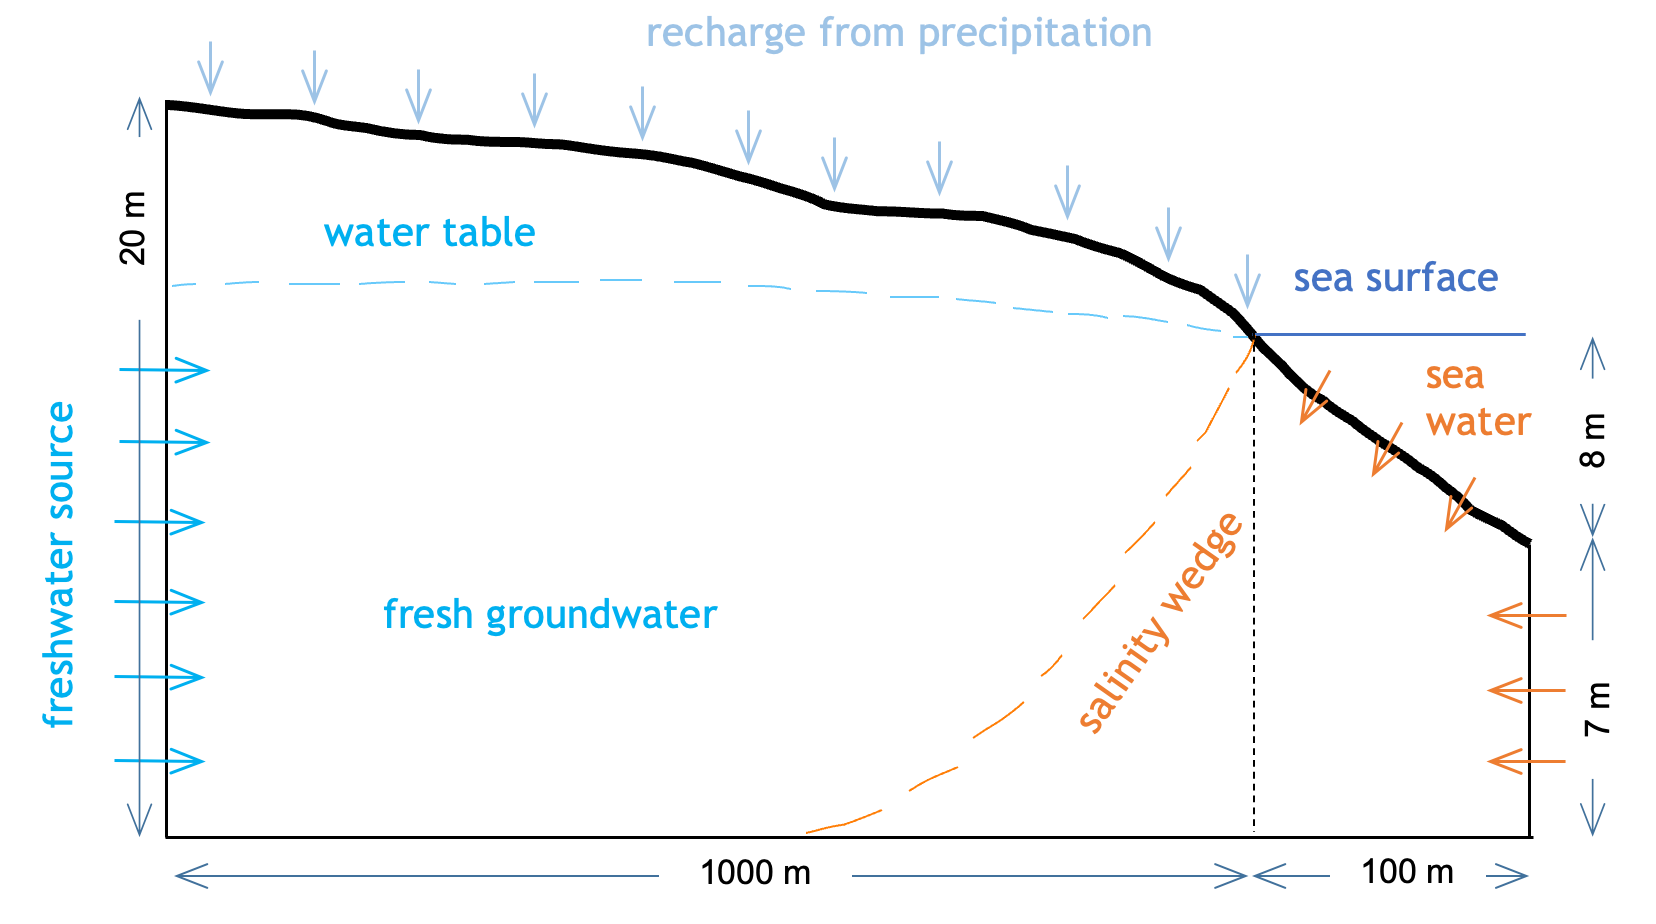
\includegraphics[width=0.75\linewidth]{figures/norfolk_domain.png}
  \caption{Schematic of the idealized 2D coastal aquifer model used in the PFLOTRAN simulations. The domain is 1100~m wide and 20~m tall, with a structured grid of 220~$\times$~200 cells. The land and offshore-shelf elevation profiles are shown, along with the location of the freshwater boundary and the offshore boundary.}
  \label{fig:grid}
\end{figure}

The 2000-member ensemble is populated by randomized batches of \texttt{NorfolkModel} realizations using \texttt{NorfolkEnsemble.draw()}, and is designed to generate a diverse set of scenarios from physically plausible distributions by varying four categories of input parameters per realization, as listed below.

\begin{itemize}
  \item \textbf{Subsurface permeability/porosity}. A single realization of a
    2D Gaussian random field is drawn with \texttt{gstools}'
    \texttt{SRF} class \citep{muller2022gstools} over an exponential covariance model (\texttt{gs.Exponential}, unit variance, length scales $[25,\,2]$~m in
    $x$ and $z$, zero rotation angle), evaluated on the model's own
    structured $N_x \times N_z$ node positions and seeded from the
    ensemble's \texttt{MasterRNG} stream for reproducibility. The same field  is used for both material properties, so that permeability and porosity are correlated across realizations. The permeability field uses a log-affine map given by $\mathrm{perm}_x = \exp(\mathrm{GRF}\cdot\sigma_{\mathrm{perm}} + \mu_{\mathrm{perm}})\times 10^{-11}$ (with $\mu_{\mathrm{perm}}=4.5$, $\sigma_{\mathrm{perm}}=0.5$ by default), and anisotropy is enforced by fixing the vertical permeability to be a fraction of the horizontal permeability, such that $\mathrm{perm}_z = 0.1\, \mathrm{perm}_x$. The porosity field is defined using a plain affine map with a physical floor,
    $\mathrm{poro} = \max(\mathrm{GRF}\cdot\sigma_{\mathrm{poro}} +
    \mu_{\mathrm{poro}},\, 0)$ (with $\mu_{\mathrm{poro}}=0.5$,
    $\sigma_{\mathrm{poro}}=0.05$ by default).
  \item \textbf{Land and offshore-shelf elevation profiles}. Two independent
    profiles are generated for the land elevation and the offshore-shelf elevation by a bounded random walk. The land profile runs from the fixed left-edge elevation ($z=5$~m) down to mean sea level ($z=0$~m) over the 1000~m inland span, and the shelf profile continues from mean sea level down to a fixed slope elevation ($z=-8$~m) over the remaining 100~m. Each walk samples one grid row per $x$-column, bounded at every interior step 
    to within $\pm 3$ vertical cells of the previous column. This is further clipped to a pair of logarithmically tapering envelopes that pinch the walk toward its fixed endpoints over the first/last 50 cells. The increments for every $x$-column are drawn from a local \texttt{RandomState} seeded off \texttt{MasterRNG}, keeping this draw reproducible in isolation. The raw walk is then smoothed with a moving average (window up to 21 cells, narrowing near the domain edges) and converted from grid-cell indices back to physical elevation before being written into the model.
  \item \textbf{Offshore salinity boundary conditions}. For every realization, twelve monthly salinity values are drawn via one independent
    \texttt{scipy.stats.uniform} draw per calendar month, from ranges based on realistic seasonal extrema. After converting to mol~NaCl~kg$^{-1}$ units, as expected by PFLOTRAN's transport constraints, the same twelve values are then tiled unchanged across every simulated year of the post-spinup simulation horizon. Thus, the seasonal cycle repeats identically year over year, with no interannual variability, and is written out as one \texttt{Sal <value> T} concentration constraint per output timestep.
  \item \textbf{Recharge and other boundary conditions}. Three further
    scalars/series are drawn per realization in the same
    \texttt{MasterRNG}-seeded fashion as the salinity record. Surface
    recharge is given by a single draw from a uniform distribution,
    $q_{\mathrm{recharge}}\sim\mathcal{U}(1\times10^{-9},\,5\times10^{-8})$~m~yr$^{-1}$, held constant for the entire realization. It is written into a 12-row monthly file for format compatibility with the deck's expected
    input. A freshwater water-table gain above mean sea level is defined for every realization through a single draw,
    $\Delta h_{\mathrm{sea}}\sim\mathcal{U}(0.5,\,2.5)$~m, and is imposed as a proxy for freshwater head strength at the offshore boundary. To account for seasonal atmospheric variability, twelve monthly values representing sea-level air pressure fluctuations are drawn in a similar fashion to salinity for every realization. These twelve independent
    $\mathcal{U}(99365,\,103285)$~Pa values (i.e.\ $101325~\mathrm{Pa}\pm
    0.2\,\rho_{\mathrm{fresh}} g \times 1~\mathrm{m}$) are repeated across the
    post-spinup years without any interannual variations.
\end{itemize}

The hydrostatic pressure at each boundary is built from these draws by a single
shared routine, $p(\mathrm{elevation}) = p_{\mathrm{ref}} + \rho g
(\mathrm{elevation}_{\mathrm{ref}} - \mathrm{elevation})$, evaluated at cell
bottoms and written as PFLOTRAN \texttt{DATASET} HDF5 files. The full-depth
\texttt{Creek} face (left boundary) uses freshwater density referenced at
mean sea level plus the $\Delta h_{\mathrm{sea}}$ head offset, and is applied
as a \texttt{DIRICHLET LIQUID\_PRESSURE} condition with \texttt{LINEAR} time
interpolation. The \texttt{Sea} face (right boundary below the shelf break at $z=-8$~m) uses saltwater density. The top boundary is split between seawater and land regions. During spin-up, the seawater region (\texttt{Wetted}) consists of the top cells below mean sea level. During the post-spinup phase it is replaced by the \texttt{Coastal} region, which has a fixed extent that accounts for all top cells below the terminal sea level, $\mathrm{MSL} + \mathrm{sea\_level\_anomaly\_rate}\cdot T = \mathrm{MSL} + 0.3$~m (using the default rate of $0.01$~m~yr$^{-1}$ over the 30-year post-spinup period). \texttt{Coastal} therefore also contains land cells that are progressively inundated. Its pressures vary monthly and are referenced against the monthly-rising sea level ($\mathrm{MSL} + \mathrm{sea\_level\_anomaly\_rate}\cdot t$) and the corresponding monthly timeseries of air-pressure variations, rather than a fixed reference. This means that cells that are already below the sea level use saltwater density, and those not yet submerged use freshwater density. This is also the mechanism through which sea-level rise is imposed during the post-spinup period. The \texttt{Recharge} region is the remaining land part of the top boundary (above mean sea level in spin-up, above the terminal sea level post-spinup). It is described by a \texttt{NEUMANN LIQUID\_FLUX} condition with \texttt{STEP} interpolation, and reads the constant $q_{\mathrm{recharge}}$ value described above.

Every random draw in the ensemble including the subsurface field, the elevation
random walks, the salinity and sea air-pressure variations, freshwater head gain, and the recharge flux is keyed off a single \texttt{MasterRNG(seed=20201007)} stream, so a given seed determines the full ensemble. However, reproducibility is order-dependent and not fully unconditional as \texttt{master\_rng()} hands out the next integer from one \texttt{RandomState} sequence. Thus, adding, removing, or reordering any draw call shifts every seed drawn after it, changing the resulting realizations even with the same seed value.

\subsubsection{PFLOTRAN input deck generation}

A separate writer module, \texttt{pfwrite}, translates a populated
\texttt{NorfolkModel} into the full set of files PFLOTRAN needs to run:
region/strata HDF5 datasets, permeability/porosity HDF5 datasets, pressure
and salinity boundary time series (HDF5), and text control decks. All
\texttt{pint}-tagged quantities are explicitly stripped of units immediately
before being written as raw floats (via a small \texttt{\_magnitude()}
helper that checks for and eliminates any silent unit-registry mismatch
errors).

The PFLOTRAN \citep{hammond2012pflotran} configuration is fixed across
the ensemble and reflects a specific, non-default feature combination:
\texttt{RICHARDS} flow coupled to \texttt{GIRT} transport, with salinity
carried as an auxiliary species (NaCl, molar mass 58.442469~g/mol) rather
than as a full reactive-transport system, and a Batzle--Wang correlation
(\texttt{EOS WATER DENSITY/VISCOSITY BATZLE\_AND\_WANG}) supplying the
density and viscosity dependence on salinity and temperature needed for the
variable-density flow and transport formulation underlying
\texttt{GIRT} \citep{lichtner2014multiscale}. Unsaturated flow
uses van Genuchten characteristic curves
($M = 0.17355$, $\alpha = 1.63\times10^{-4}$, residual liquid saturation
$0.10$, Mualem permeability function). As discussed before, each realization is set up to run in two stages: a 10-year spin-up to establish an initial hydrostatic/steady salinity distribution, followed by a checkpoint-restarted post-spin-up run forced by time-varying sea- and land-surface boundary pressures that encode a prescribed sea-level-rise trajectory. 

An extensive \texttt{pytest} suite (\texttt{src/pflotran\_swi/tests}) is included to ensure correctness of the writer. This verifies unit handling, ensemble metadata (a small \texttt{NorfolkModelList} subclass added so that
\texttt{NorfolkEnsemble.draw()} output retains a case name), and
notebook-level end-to-end execution.

\subsubsection{Neural-operator surrogate architecture}

The archived simulation ensemble (\S\ref{sec:findings}) is used as the training/test data for \texttt{SWINet}, a separate, actively developed repository implementing a MITONet-style neural operator \citep{riveracasillas2026mitonet}. This architecture features independent branch networks that encode static and
time-windowed input fields, and a trunk network that encodes query
coordinates/time. The outputs of these branch and trunk networks are combined via a structured inner product to produce the desired predicted field.
The architecture was adapted from the MITONet implementation provided in the  (\texttt{UT-CHG/SW\_MITONet}) GitHub repository \citep{dutta2026swmitonet},
by bypassing the separate autoencoder stage to directly read the 2D structured grid data fields as input to the branch networks $(n_z, n_x, 1)$ using 2D convolutional layers. Two variants are implemented and are being actively developed in parallel, with different trade-offs between rollout speed and per-step accuracy:

\begin{itemize}
  \item \textbf{SWINet} predicts one look-forward step $t_0 + \tau$ per
    forward pass. This is achieved through an autoregressive rollout that uses a heap-based event scheduler so that each state variable can advance on its own $\tau$ cadence while still reading every other variable's latest state as a cross-variable initial condition.
  \item \textbf{SWINetTensorT} is an alternative variant that uses temporal bundling to predict an entire block of $\tau$ steps in one forward pass. This is implemented using a split trunk (a spatial sub-network plus a tensorized temporal sub-network). The autoregressive rollout is designed as a simpler lockstep loop since the trained \texttt{tensort} model for each state variable is constrained to predict the same $\tau$-step block.
\end{itemize}

Both variants share the same 14-branch input set incorporating static permeability, porosity, elevation, model parameters, and creek boundary condition; windowed initial conditions for pressure, $v_x$, $v_z$, salinity, and
saturation; as well as windowed boundary forcing for the sea face, the coastal top (offshore-shelf) boundary, groundwater-recharge, and salinity boundaries. The models are trained to predict the five state variables at $t_{\mathrm{skip}} = 8$-snapshot cadence (roughly 30 days), generating about 286
snapshots per 25-year simulation. In the preliminary results, \texttt{saturation} has no trained model in either architecture and is always read from ground truth during rollout. 

One of the primary challenges of data-driven, neural operator-based modeling of the flow characteristics of coastal seawater intrusion is the difficulty of accurately capturing the sharp transitions in the salinity fields. To address this challenge, the training process for SWINet and SWINetTensorT supports three optional modifications. Let $y$ denote a target state variable on the grid, $\hat{y}$ the network prediction, and $m_{ij}\in\{0,1\}$ a mask selecting the active (subsurface) cells, with $i$ and $j$ the vertical and horizontal cell indices. The baseline loss function is the masked mean squared error,
$\mathcal{L}_{\mathrm{val}} = \sum_{ij} m_{ij}(\hat{y}_{ij}-y_{ij})^2 \big/ \sum_{ij} m_{ij}$.

\emph{Front-weighted MSE} keeps this value-matching form but reweights each cell by how steep the true field is around it,
\begin{equation}
  \mathcal{L}_{\mathrm{val}} =
  \frac{\sum_{ij} w_{ij}\, m_{ij}\,(\hat{y}_{ij}-y_{ij})^2}{\sum_{ij} w_{ij}\, m_{ij}},
  \qquad
  w_{ij} = 1 + \lambda\,\frac{|\delta_z y_{ij}| + |\delta_x y_{ij}|}{\max_{kl}\left(|\delta_z y_{kl}| + |\delta_x y_{kl}|\right)},
  \label{eq:front-weight}
\end{equation}
where $\delta_z$ and $\delta_x$ are finite difference approximations of the gradients between neighboring cells in the vertical and horizontal directions and $\lambda\ge 0$ sets the strength of the reweighting (such that $\lambda=0$ recovers the plain MSE). The weights are computed from the ground truth alone, so they act purely as a static emphasis map: errors near the front count up to $1+\lambda$ times more than errors in the uniform regions, but the loss still compares only field values.

\emph{Sobolev loss}, in contrast, adds a separate term that compares the spatial gradients of the prediction and the truth,
\begin{equation}
  \mathcal{L} = \mathcal{L}_{\mathrm{val}} + \beta\,
  \frac{\sum_{ij} m_{ij}\left[(\delta_z\hat{y}_{ij}-\delta_z y_{ij})^2 + (\delta_x\hat{y}_{ij}-\delta_x y_{ij})^2\right]}{\sum_{ij} m_{ij}},
  \label{eq:sobolev}
\end{equation}
with $\beta\ge0$ weighting the gradient mismatch against the value mismatch. A front that is smeared out or displaced by a few cells produces a small value error at each affected cell but a large gradient error where the transition should be, so this term penalizes such errors directly rather than through a reweighting proxy. In practice $\beta$ is ramped up from zero over the first few epochs so that the network first learns the coarse field before being asked to match its gradients. The two modifications are complementary and can be used together. For instance, the best performing salinity models tested in the preliminary analysis use $\lambda=2$ and $\beta=1$.

\emph{Initial-condition noise injection} addresses a different failure mode. During an autoregressive rollout the network's own predictions are fed back in as the initial condition for the next step, so any error is compounded from step to step, whereas during training the initial conditions are always the ground truth simulation output.
To narrow this gap, small zero-mean Gaussian perturbations are added to the initial-condition inputs of a random fraction of the training samples (the perturbation amplitude is a few percent of the normalized data range, and it
can be ramped up gradually like $\beta$), and the perturbed inputs are clipped to the valid range. The target is left unperturbed, so the network learns to map slightly-off states back toward the true evolution, which reduces the
error accumulation and the occasional divergence of rollouts.

\subsection{Preliminary Results and Analysis}
\label{sec:findings}

Here we present findings from a preliminary analysis conducted using a randomly drawn sample of 350 PFLOTRAN simulations from the generated 2000-member enesemble, where each realization is an independent, 25-year post-spin-up simulation produced by this pipeline. The results of the neural operator approximation are obtained using the current best model configuration for each state variable using either the SWINet or SWINetTensorT architecture. The surrogate model is evaluated on a held-out test split of 30 cases, and the reported metrics are averaged over these cases. The surrogate model's performance is assessed using normalized root mean square error (NRMSE) and anomaly correlation coefficient (ACC) metrics.
% All quantities reported here were computed directly from the
% raw per-case HDF5/text output rather than from any pre-aggregated summary,
% since -- as documented in the SWINet repository's own
% \texttt{ensemble\_params.csv} -- most sampled per-case parameters are not
% stored anywhere as scalars and must be reconstructed from the simulation
% output itself (e.g., the land/shelf elevation profile has to be recovered
% from the topmost active-material cell per grid column, and the boundary
% salinity forcing from the constraint-file text rather than any array on
% disk).

\subsubsection{Simulation ensemble characteristics}

Figure~\ref{fig:ensemble-spread} summarizes the realized spread of four
ensemble parameters across all 350 available realizations: mean
$\log_{10}$(permeability$_x$), mean porosity, mean land/shelf surface
elevation, and mean boundary salinity forcing. All four show continuous,
unimodal coverage rather than degenerate or clustered sampling -- the
permeability, porosity, and salinity panels are roughly symmetric and
bell-shaped, while the elevation panel is right-skewed, consistent with the
land-profile random walk's fixed endpoints (5~m at the inland edge, 0~m at
the shore) constraining how much of the realized mean can sit near the
lower end. This is the expected signature of the underlying
Gaussian-random-field and bounded-random-walk generators operating
correctly across the ensemble.

\begin{figure}[htbp]
  \centering
  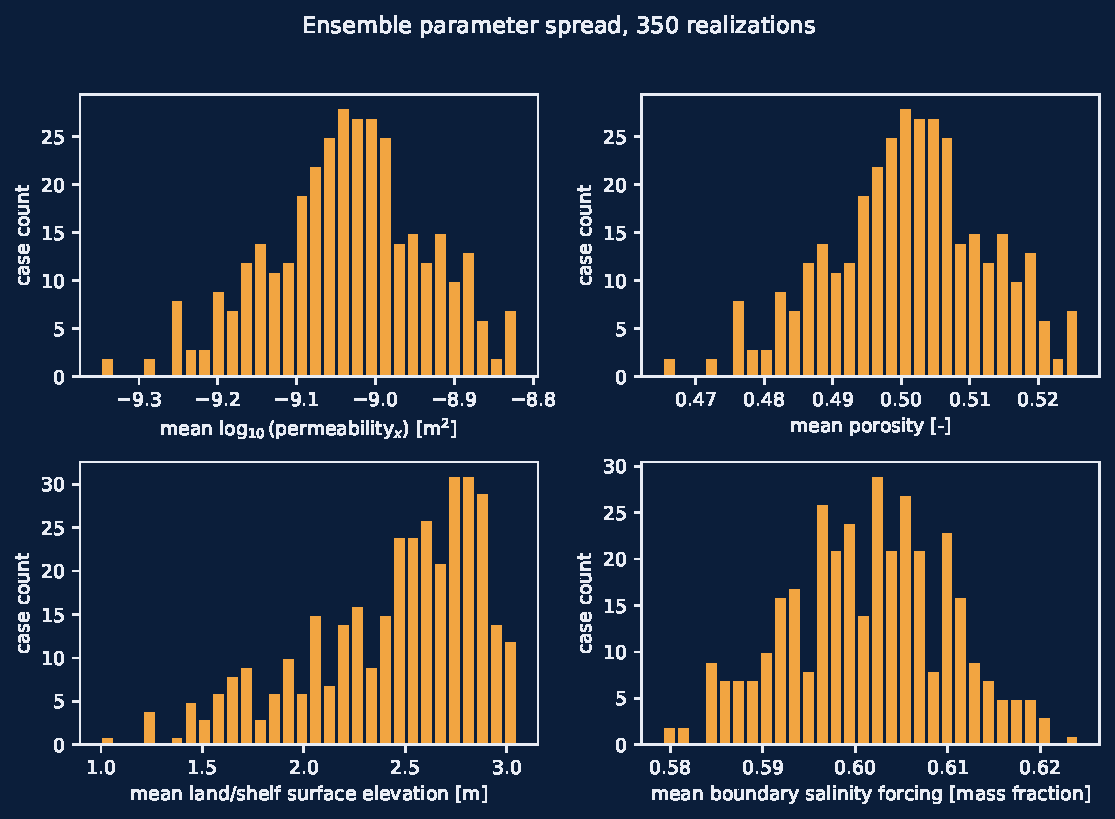
\includegraphics[width=0.75\linewidth]{figures/fig2_ensemble_spread.pdf}
  \caption{Ensemble parameter spread across 350 archived realizations.
    Each panel shows the distribution of the mean value per realization for one parameter across the ensemble. }
  \label{fig:ensemble-spread}
\end{figure}

\subsubsection{Permeability field realizations}

Figure~\ref{fig:perm-realizations} shows the spatial structure of the
anisotropic sampled permeability field for five random \texttt{NorfolkEnsemble}
realizations. Each panel plots the harmonic mean of
$\mathrm{perm}_x$ and $\mathrm{perm}_z$, masked to the
active (below-ground/below-seabed) cells, so the visible outline is the
same land/shelf profile driving that realization's flow boundary
conditions. The exponential-covariance correlation structure, defined by $x,z$ length scales of $25$~m and $2$~m, respectively, is visible
as a mottled, patchy texture with mild horizontal elongation rather than
isotropic speckle or discernible stratification. The distinct spatial features at both the field level and the terrain across the five random realizations provides qualitative evidence that the correlated permeability/porosity sampling method and the independent land/shelf elevation walk described in \S\ref{sec:methodology} are producing distinct, spatially structured realizations.

\begin{figure}[htbp]
  \centering
  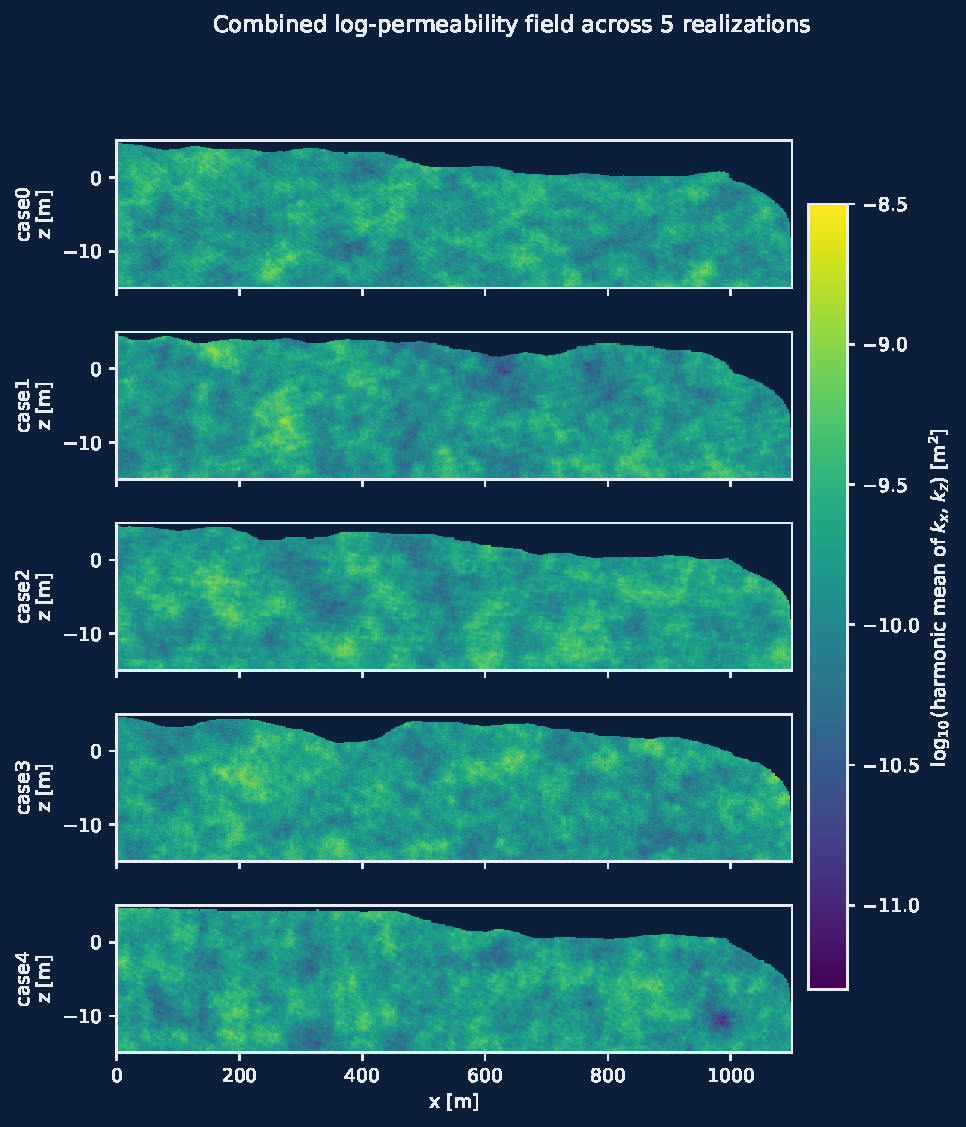
\includegraphics[width=0.75\linewidth]{figures/fig2b_permeability_realizations.pdf}
  \caption{Combined log-permeability field (harmonic mean of
    $\mathrm{perm}_x$, $\mathrm{perm}_z$; $\log_{10}$, m$^2$) for five
    realizations, masked to active (subsurface) cells. Vertical axis
    exaggerated $12\times$ relative to the horizontal.}
  \label{fig:perm-realizations}
\end{figure}

\subsubsection{Representative intrusion dynamics}

Figure~\ref{fig:intrusion-evolution} shows the salinity field for a single
representative simulation (case 1) at three points in the post-spin-up horizon:
initial condition, roughly the midpoint (T~$\approx$~12.5~yr), and the final
archived time (T~$\approx$~25.0~yr). The wedge advances from a narrow zone
confined to the offshore/creek boundary at $T=0$ to occupying essentially
the entire bottom half of the domain by the final snapshot, consistent with
the intended sea-level-rise-driven intrusion scenario the ensemble was
designed to sample.

\begin{figure}[htbp]
  \centering
  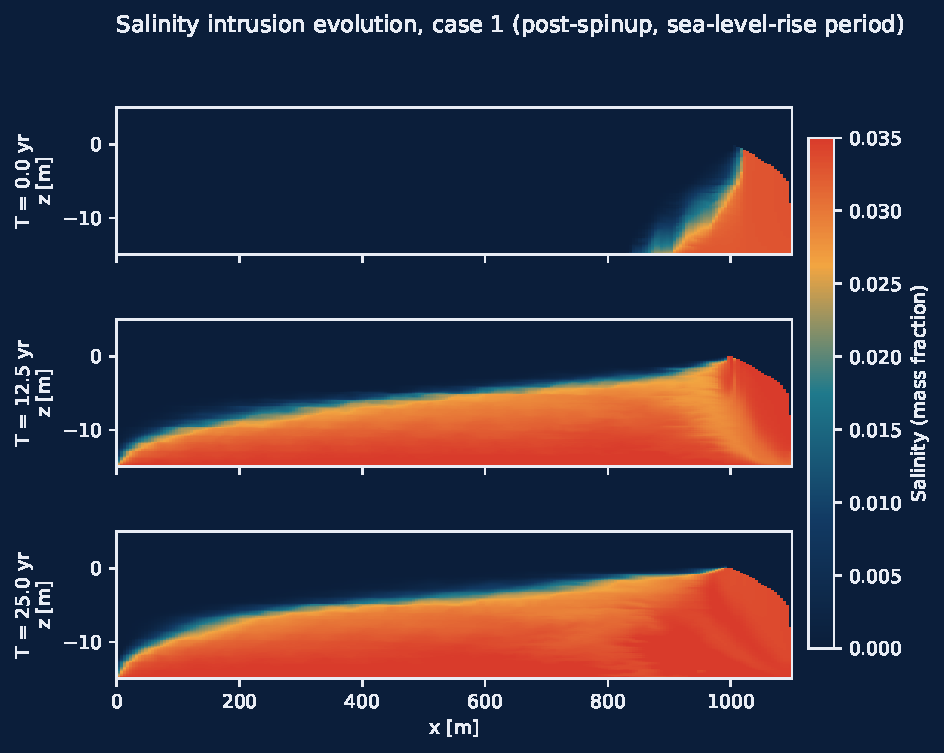
\includegraphics[width=0.7\linewidth]{figures/fig1_intrusion_evolution.pdf}
  \caption{Salinity intrusion evolution for case 1 across the post-spin-up
    simulated horizon. Vertical axis exaggerated $12\times$ relative to the
    horizontal for legibility, matching the domain aspect used in
    \texttt{condensed\_slides.pdf}.}
  \label{fig:intrusion-evolution}
\end{figure}

Figure~\ref{fig:multi-realization} compares the salinity field at the
\emph{final} archived time across five realizations spanning the
permeability distribution in Figure~\ref{fig:ensemble-spread} (cases 1, 75,
150, 225, 300). The differences between cases at this late time are
noticeably subtler than the within-case evolution shown in
Figure~\ref{fig:intrusion-evolution}: by 25 years, most sampled parameter
combinations have driven the aquifer toward a similarly near-fully-intruded
bottom layer, with the visible across-case variation concentrated in the
transition-zone thickness and the toe slope rather than in the total extent
of intrusion. This suggests that, at the ensemble's simulated horizon, the
distinguishing signal between cases lives mainly in the \emph{transient}
approach to the intruded state rather than in the endpoint -- a property
that plausibly bears on the surrogate-model error pattern discussed next.

\begin{figure}[htbp]
  \centering
  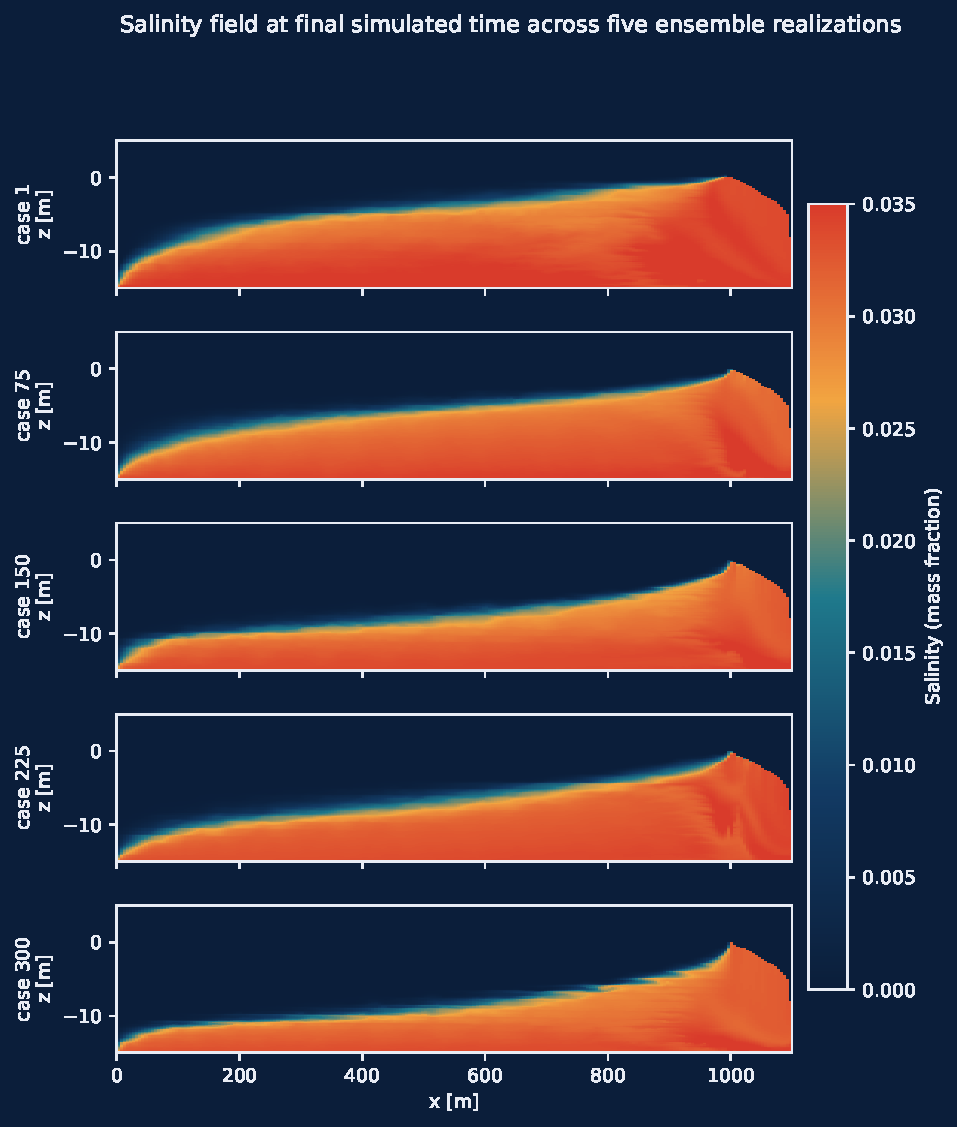
\includegraphics[width=0.7\linewidth]{figures/fig3_multi_realization.pdf}
  \caption{Salinity field at the final archived time for five realizations
    spanning the permeability range of the ensemble.}
  \label{fig:multi-realization}
\end{figure}

\subsubsection{Surrogate model performance}

Table~\ref{tab:swinet-status} summarizes the currently best-available SWINet/SWINetTensorT model for each state variable, evaluated as an average over 30 unseen test cases.

\begin{table}[htbp]
  \centering
  \caption{Best available SWINet/SWINetTensorT model by state variable (30-case
    test-split average).}
  \label{tab:swinet-status}
  \begin{tabular}{lll}
    \toprule
    Variable & Feature & NRMSE / ACC  \\
    \midrule
    pressure & \texttt{Optuna} & 0.0074 / 1.000  \\
    $v_z$ & \texttt{Optuna} & 0.0200 / 0.968   \\
    $v_x$ & \texttt{Optuna} & 0.0268 / 0.610   \\
    salinity & \texttt{Sobolev} & 0.0913 / 0.958   \\
    salinity (tensort) & \texttt{Tensort, Sobolev, ICnoise} & 0.0712 / 0.944  \\
    \bottomrule
  \end{tabular}
\end{table}

The salinity model's dominant error mode is a systemic over-prediction of intrusion rate such that the predicted salt-water toe advances roughly twice as fast as ground truth, that is currently being investigated. Similarly, the relatively lower ACC value of the $v_x$ model and the feasibility of replacing the $v_x$ and $v_z$ models with a cheaper Darcy-law derivation from the predicted pressure field are both open, actively tracked issues rather than resolved limitations of the reported numbers. 

Figure~\ref{fig:swinet-rollout} shows the \texttt{SWINetTensorT}
(using tensorized temporal bundling and Sobolev loss regularization) salinity model's autoregressive rollout against PFLOTRAN ground truth for one of the randomly chosen test cases (case 271), at the same three time points in the post-spin-up horizon as used in Figure~\ref{fig:intrusion-evolution}. Per-snapshot NRMSE for this case ranges from 0.074 to 0.082, which is consistent with the architecture comparison numbers in Table~\ref{tab:swinet-status}. 

\begin{figure}[htbp]
  \centering
  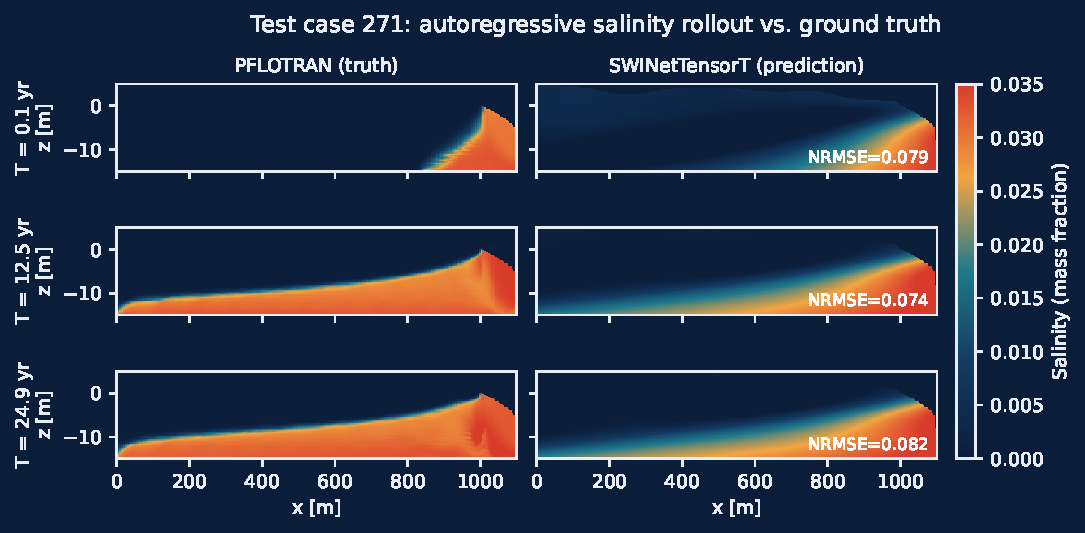
\includegraphics[width=0.85\linewidth]{figures/fig4_swinet_rollout.pdf}
  \caption{Test case 271: SWINetTensorT autoregressive salinity
    prediction vs.\ PFLOTRAN ground truth, three snapshots across the
    rollout. }
  \label{fig:swinet-rollout}
\end{figure}
